\section{Auswertung}
\subsection{Dämpfung}
Nach Gl. \ref{eqn:Absorption} beschreibt $\alpha$ den Absorbtionskoeffizenten, und
somit die Dämpfung der Intensität.
Für das Impuls-Echo-Verfahren ergibt sich für eine Länge $L$ eines Zylinders
\begin{equation}
    I(2L)=I_0e^{-\alpha 2L},
\end{equation}
mit
\begin{equation}
    \alpha=-\frac{1}{2L}\text{ln}\left(\frac{I(2L)}{I_0}\right).
\end{equation}
\begin{table}
    \centering
    \begin{tabular}{c|c c c}
        \toprule
        &Zylinder 1 &Zylinder 2&Zylinder 3\\
        \midrule
        Länge $L$ [cm] &30&40.04&120.04\\
        $I(2L)$ [V] &1.33&0.7&0.11\\
        $I_0$ [V]& 1.33&1.35&1.34\\
        $t$ [$\mu$s]&30&59.8&88.9\\
        \midrule
        $\alpha$ [cm$^{-1}$]& 0&0.004&0.01\\
        \bottomrule
    \end{tabular}
    \caption{}
    \label{tab:wertetabelle}
\end{table}

\subsection{Schallgschwindigkeitsbestimmung}
Die Bestimmung der Schallgeschwindikeit der Schallgeschwindigkeit der Anpassungschicht
der Sonde kann mithilfe der Laufzeit $t$ (siehe Tab. \ref{tab:wertetabelle}) erzielt werden.

\begin{table}
    \centering
    \begin{tabular}{c | c c c}
        \toprule
        &\multicolumn{2}{c}{Echo-Verfahren} & \multicolumn{1}{c}{Duchschall-Verfahren}\\
        \cmidrule(lr){2-3}\cmidrule(lr){4-4}
        & $t\;/\;\mu s$ &  $\frac{t}{2}\;/\;\mu s$& $t\;/\;\mu s$\\ 
        \midrule
        kleiner Zylinder & 30 & 15 & 16.4\\
        mittlere Zylinder & 59.8 &29.9 & 31.3\\
        großer Zylinder & 88.9 &44.45& 45.1\\
        \bottomrule
    \end{tabular}
    \caption{Darstellung der Laufzeiten t mit den 2. verschiedenen Verfahren.}
\end{table}

Dafür wird die Laufzeit (hier nun $\frac{t}{2}$) gegen die Länge $L$ der Zylinder aufgetragen.
\begin{figure}[H]
    \centering
    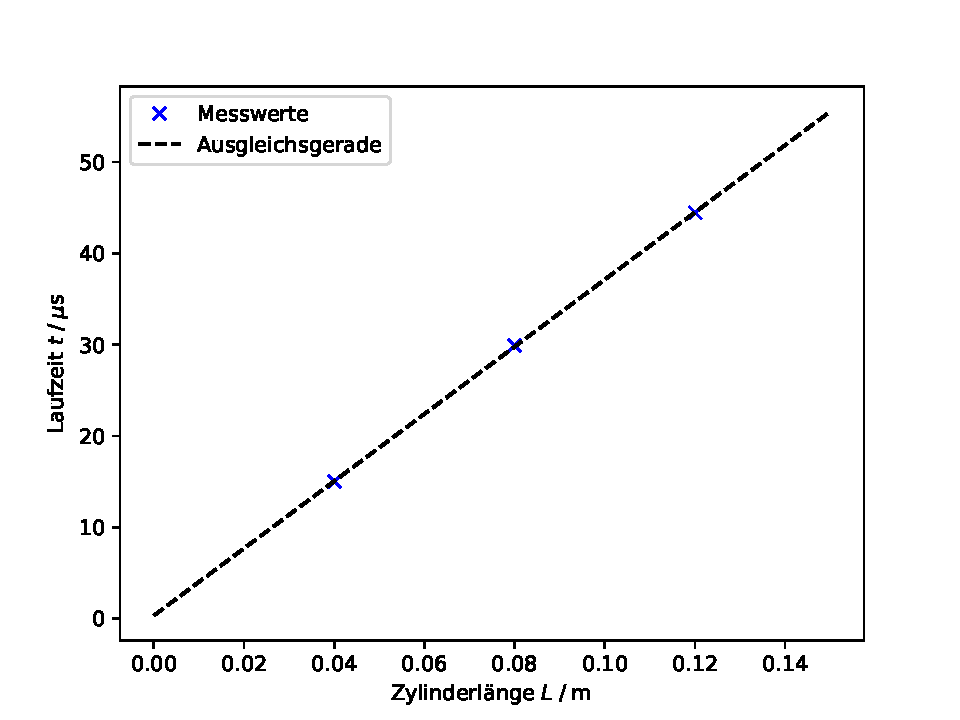
\includegraphics[width=0.8\textwidth]{plots/laufzeit_echo.pdf}
    \caption{Aufgetragen sind die Messwerte des Echo-Verfahren und eine lineare
    Ausgleichsgerade.}
\end{figure}
Über die Ausgleichsgerade, nach
\begin{equation}
    t=m \cdot L+n,
\end{equation}
lässt sich nun der y-Achsenabschnitt $n$ bestimmen.
Er spiegelt einen systematischen Fehler wieder, der aus der Dicke der Anpassungsschicht
resultiert.\\ 
Für die Parameter ergibt sich
\begin{align*}
    m=(367.99\pm2.6)\frac{\mu s}{cm},\\
    n=(0.32\pm0.23)\mu s.
\end{align*}
Über die Laufzeitgeschwindigkeit $n$ und die Schallgeschwidigkeit von Wasser
$c_{\text{Wasser}}=343m/s$ der Anpassungsschicht kann nun mit
\begin{equation}
    d=\frac{1}{2} \cdot c_{\text{wasser}} \cdot n,
\end{equation}
die Dicke $d$ der Anpassungschicht mit
\begin{equation}
    d=55.9\mu m
\end{equation}
angegeben werden.
Für die angepasste Schallgeschwindikeit in Acyril ergibt über den 
Kehrwert des Steigungsparameter $m$ die Acyrilschallgeschwindigkeit $c_{echo,acyril}$ mit,
\begin{equation}
    c_{\text{echo,acyril}}=(2717\pm19)\frac{m}{s}
\end{equation}

Analoges Vorgehen folgt für die Durchschallungs-Methode.
\begin{figure}[H]
    \centering
    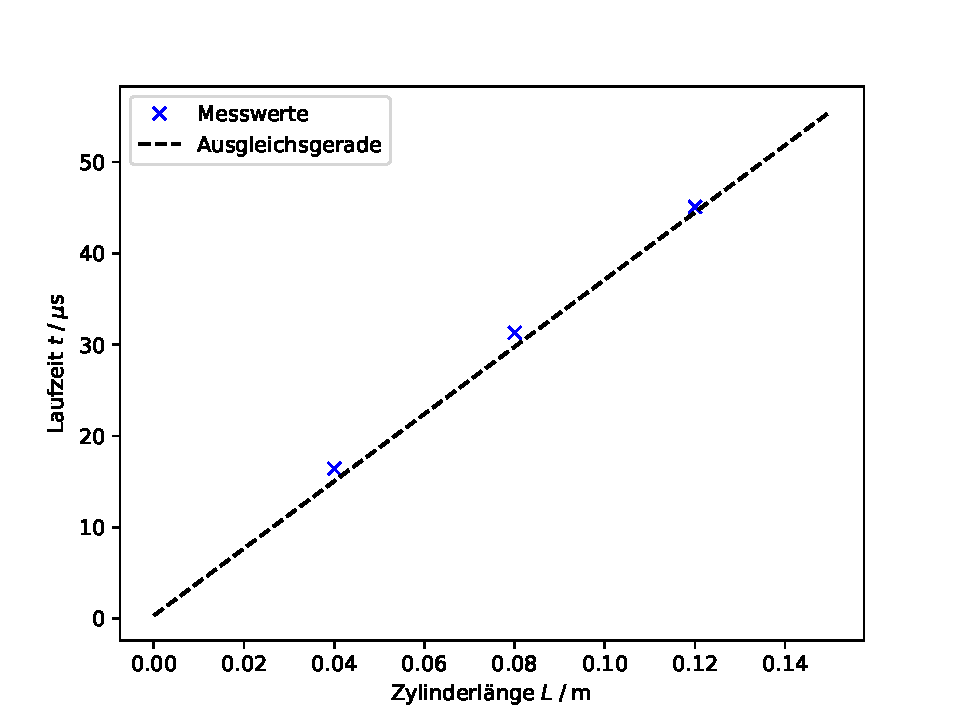
\includegraphics[width=0.8\textwidth]{plots/laufzeit_durch.pdf}
    \caption{Aufgetragen sind die Messwerte des Durchschallungs-Verfahren und eine lineare
    Ausgleichsgerade.}
\end{figure}

Für die Regressionsparamter folgt,
\begin{align*}
    m&=(359\pm8)\frac{\mu s}{m},\\
    n&=(2.2\pm0.7)\mu s,\\
\end{align*}
und somit,
\begin{equation}
    c_{\text{durch,acyril}}=(2790\pm6)\frac{m}{s}.
\end{equation}
\subsection{Biometrische Untersuchung eines Augenmodells}
Aus den vier gemessenen Peaks, kann auf Abmessung des Augenmodells zurückgeschlossen werden.
Dabei führt man den ersten Peak auf die Hornhaut, den zweiten Peak auf den Anfang der Linse, den dritten Peak
auf das Ende der Linse und den letzten Peak auf die Netzhaut zurück.\\
Zu beachten sind nun die verschiedenen Schallgeschwindigkeiten.

Für die Abstände ergeben sich folgende Formeln,
\begin{align*}
    \textrm{Hornhaut - Anfang Linse}:& &s_1&=\frac{1}{2}c_1t_1,\\
    \textrm{Hornhaut - Ende Linse}:& &s_2&=\frac{1}{2}c_2(t_2-t_1)+s_1,\\
    \textrm{Hornhaut-Netzhaut}:& &s_3&=\frac{1}{2}c_2(t_3-t_2)+s_2,\\
\end{align*}
mit den jeweiligen Geschwindigkeiten,
\begin{align*}
    \text{Kammerflüssigkeit}: & &c_1=1532 m/s,\\
    \text{Linsenmaterial}: & &c_2=2500 m/s,\\
    \text{Glaskörperflüssigkeit}: & &c_3=1410 m/s
\end{align*}
\begin{table}
    \centering
    \begin{tabular}{c| c c}
        \toprule
        & Zeit $t\;/\;\mu$s&Abstand $s\;/\;10^{-3}$m\\
        \midrule
        Anfang Linse (Iris) &11.5& 4.4\\
        Ende Linse &17& 7.8\\
        Netzhaut &70.6& 26.7\\
        \bottomrule
    \end{tabular}
    \caption{Darstellung der Messzeit $t$ mit dem Impuls-Echoverfahren und die daraus
    resultierenden Abmessungen.}
\end{table}
\label{sec:Auswertung}
